\documentclass[a4paper,12pt,french]{article}

\usepackage[utf8]{inputenc}
\usepackage[T1]{fontenc}
\usepackage{lmodern}
\usepackage{kpfonts}
\usepackage[margin=1.4cm]{geometry}
\usepackage{amsmath,amsfonts,amssymb}
\usepackage{enumitem}
\usepackage{tikz}
\usetikzlibrary{intersections}

\usepackage[np]{numprint}

\usepackage{babel}
\usepackage[]{exercise}

\setlist{noitemsep}
%\setlist[1]{\labelindent=\parindent} % < Usually a good idea
\setlist[itemize]{leftmargin=*}
\setlist[itemize,1]{label=$\triangleright$}
\setlist[enumerate]{labelsep=*, leftmargin=1.5pc}
\setlist[enumerate,1]{label=\arabic*., ref=\arabic*}
\setlist[enumerate,2]{label=\emph{\alph*}),
ref=\theenumi.\emph{\alph*}}
\setlist[enumerate,3]{label=\roman*), ref=\theenumii.\roman*}
\setlist[description]{font=\sffamily\bfseries}

\renewcommand{\ExerciseName}{Exercice}
\renewcommand{\AnswerName}{Réponse de l'exercice}

\newcommand{\N}{\mathbf{N}}
\renewcommand{\u}{(u_n)_{n\in\N}}

\everymath{\displaystyle\everymath{}}

\title{D.S. 1}
\date{7 octobre 2015}

\begin{document}

\maketitle

\begin{Exercise}[number=1]
  Soit $(u_n)_{n\in\N}$ la suite définie par $u_0 = 5$ et pour tout
  nombre entier naturel $n$, par \[u_{n+1} = \frac{4u_n - 1}{u_n+2}.\]
  Si $f$ est la fonction définie sur l'intervalle $]-2;+\infty[$ par \[
  f(x) = \frac{4x -1}{x+2}, \] alors on a pour tout entier naturel,
  $u_{n+1} = f(u_n)$. On donne en annexe une partie de la courbe
  $\mathcal{C}_f$ de la courbe de la fonction $f$ ainsi que la droite
  $\delta$ d'équation $y=x$.

  \begin{enumerate}
    \item \begin{enumerate}
        \item Sur l'axe des abscisses, placer $u_0$ puis construire
          $u_1$, $u_2$ et $u_3$ en laissant apparents les traits de
          construction.
        \item Quelles conjectures peut-on emettre sur le sens de
          variation et sur la convergence de la suite $(u_n)_{n\in\N}$ ?
      \end{enumerate}
    \item \begin{enumerate}
        \item Démontrer par récurrence que, pour tout nombre entier
          naturel, $\ u_n -1 > 0$.

        \item \emph{Dans cette question toute trace de recherche, même
            incomplète ou d'initiative même non fructueuse sera prise en
          compte dans l'évaluation.}

          Valider par une démonstration les conjectures émises à la
          question 1.b)
      \end{enumerate}
    \item Dans cette question, on se propose d'étudier la suite
      $(u_n)_{n\in\N}$ par une autre méthode, en déterminant une
      expression de $u_n$ en fonction de $n$.

      Pour tout nombre entier naturel, on pose \[ v_n = \frac1{u_n -1}.
      \]
      \begin{enumerate}
        \item Démontrer que la suite $(v_n)_{n\in\N}$ est une suite
          arithmétique de raison $\frac13$.

        \item Pour tout nombre entier naturel, exprimer $v_n$ puis $u_n$
          en fonction de $n$.

        \item En déduire la limite de la suite $(u_n)_{n\in\N}$.
      \end{enumerate}
  \end{enumerate}

\end{Exercise}

\begin{Exercise}[number=2]
  En prévision d'une élection entre deux candidats $A$ et $B$ d'une
  ville, un institut de sondage recueille les intentions de vote des
  futurs électeurs.

  Parmi les \np{1200} personnes qui ont répondu au sondage, \np[\%]{47}
  affirment vouloir voter pour le candidat $A$ et les autres pour le
  candidat $B$.

  Compte-tenu du profil des candidats, l'institut de sondage estime
  que \np[\%]{10} des personnes déclarant vouloir voter pour le
  candidat $A$ ne disent pas la vérité et votent en réalité pour le
  candidat $B$, tandis que \np[\%]{20} des personnes déclarant voter
  pour le candidat $B$ ne disent pas la vérité et votent en réalité
  pour le candidat $A$.

  On choisit au hasard une personne ayant répondu au sondage et note :
  \begin{itemize}%[label=\textbullet]
    \item $A$ l'événement « la personne interrogée affirme vouloir
      voter pour le candidats $A$ » ;
    \item $B$ l'événement « la personne interrogée affirme vouloir
      voter pour le candidat $B$ » ;
    \item $V$ l'événement « la personne interrogée dit la vérité ».
  \end{itemize}

  \begin{enumerate}
    \item Construire un arbre de probabilité traduisant la situation.
    \item \begin{enumerate}
        \item Calculer lal probabilité que la personne interrogée dise
          la vérité.
        \item Sachant que la personne interrogée dit la vérité,
          calculer la probabilité qu'elle affirme vouloir voter pour
          le candidat $A$.
      \end{enumerate}
    \item Démontrer que la probabilité que la personne choisie vote
      effectivement pour le candidat $A$ et de \np{0.529}.

  \end{enumerate}

\end{Exercise}

\begin{Exercise}[number=3]
  Soit la suite numérique $(u_n)_{n\in\N}$ définie par $u_0 = 2$ et,
  pour tout entier naturel $n$ par \[ u_{n+1} = \frac15u_n + 3 \times
  \np{0.5}^n. \]
  \begin{enumerate}
    \item \begin{enumerate}
        \item Démontrer, par récurrence, que pour tout entier naturel
          non nul, on a : \[ u_n \geqslant \frac{15}4 \times
          \np{0.5}^n.\]
        \item En déduire, que pour tout entier naturel non nul, \[
          u_{n+1} - u_n \leqslant 0.\]
        \item Démontrer que la suite $(u_n)_{n\in\N}$ est convergente.
      \end{enumerate}
    \item On se propose dans cette question de déterminer la limite de
      la suite $(u_n)_{n\in\N}$.

      Soit $(v_n)_{n\in\N}$ la suite définie sur $\N$ par $v_n = u_n -
      10\times \np{0.5}^n$.
      \begin{enumerate}
        \item Démontrer que la suite $(v_n)_{n\in\N}$ est une suite
          géométrique de raison $\frac15$. On précisera le premier terme
          de la suite $(v_n)_{n\in\N}$.
        \item En déduire, que pour tout entier naturel, $u_n = -8 \times
          \left(\frac15\right)^n + 10\times \np{0.5}^n$.
        \item Déterminer la limite de la suite $(u_n)_{n\in\N}$.
      \end{enumerate}
  \end{enumerate}
\end{Exercise}

\pagebreak
Nom:

Prénom :

\vspace{1cm}
\hfill
\begin{tikzpicture}[rotate=-90,scale=4]
  \draw[very thin, lightgray] (-0.3,-0.3) grid [step=0.5] (5.7,3.6) ;
  \draw[thick,green] plot [domain=0.1:5.7] (\x,{(4*\x-1)/(\x+2)}) node
  [rotate=-90,right,black] { $\mathcal{C}_f$ } ;
  \draw[thick] plot [domain=-0.3:3.6] (\x,\x) node[rotate=-90,right] {
  $\Delta$ } ;
  \draw[->] (-0.3,0) -- (5.7,0) ; \draw [->] (0,-0.3) -- (0,3.6) ;
  \foreach \x in {0.5,1,...,5.5} {
    \draw (\x,0) -- (\x,-0.02) node [below,fill=white,rotate=-90] {
    \scriptsize \np{\x} } ;
  }
  \foreach \y in {0.5,1,...,3.5} {
    \draw (0,\y) -- (-0.02,\y) node [left,fill=white,rotate=-90] {
    \scriptsize \np{\y} } ;
  }
  \draw (0,0) node[below right,rotate=-90] { \scriptsize 0} ;
  \draw (0,0) node[above left,rotate=-90] { \scriptsize 0} ;
\end{tikzpicture}
\hfill~

\pagebreak

\begin{Answer}[number=1]
  \begin{enumerate}
    \item \begin{enumerate}
        \item cf Annexe.
        \item La suite $\u$ \emph{semble} être décroissante.
      \end{enumerate}
    \item \begin{enumerate}
        \item Démontrons par récurrence que $\forall n\in\N,\ u_n -1 >
          0$.

          \begin{description}
            \item[Initialisation] $u_0 = 5$ et $5 - 1 = 4 > 0$, donc la
              proposition est vraie au rang $n$.
            \item[Hérédité] Soit $n$ un entier naturel et supposons que
              $u_n-1 > 0$

              $u_n - 1 > 0 \implies u_n + 2 > 3 > 0$

              $u_{n+1} - 1 = \frac{4u_n -1}{u_n+2} - 1 = \frac{4u_n - 1
              - u_n -2}{u_n + 2} = \frac{3(u_n -1)}{u_n+2}$

              L'hypothèse de récurrence garantit que numérateur et
              dénominateur sont positifs, donc $\boxed{u_{n+1} -1 > 0}$.
            \item[Conclusion] $\forall n \in \N,\ u_n -1 >0$
          \end{description}
        \item Montrons que la suite est décroissante, c'est à dire que
          $\forall n \in \N,\ u_{n+1} \leqslant u_n$.

          Raisonnons par équivalences successives :

          $u_{n+1} = \frac{4u_n -1}{u_n+2} \leqslant u_n \iff 4u_n -1
          \leqslant u_n^2 + 2u_n \iff 0\leqslant u_n^2 - 2u_n +1 = (u_n
          -1)^2$. Cette dernière affirmation étant toujours vraie, on a
          la décroissance conjecturée.
      \end{enumerate}
    \item \begin{enumerate}
        \item Démontrons que $(v_n)_{n\in\N}$ est une suite
          arithmétique.

          $v_{n+1} - v_n = \frac1{u_{n+1}-1} - \frac1{u_n -1} =
          \frac{\frac13(u_n + 2)}{u_n -1 } - \frac1{u_n -1} =
          \frac{\frac13 u_n - \frac13}{u_n -1} = \frac13$.

          La suite est donc arithmétique de raison $\frac13$.

        \item $v_n = \frac13 n + \frac14$

          $u_n = \frac1{v_n} + 1 = 1 + \frac1{\frac13 n + \frac14}$

        \item $\boxed{\lim_{n\to+\infty} u_n = 1}$
      \end{enumerate}
  \end{enumerate}


\vfill
\hfill
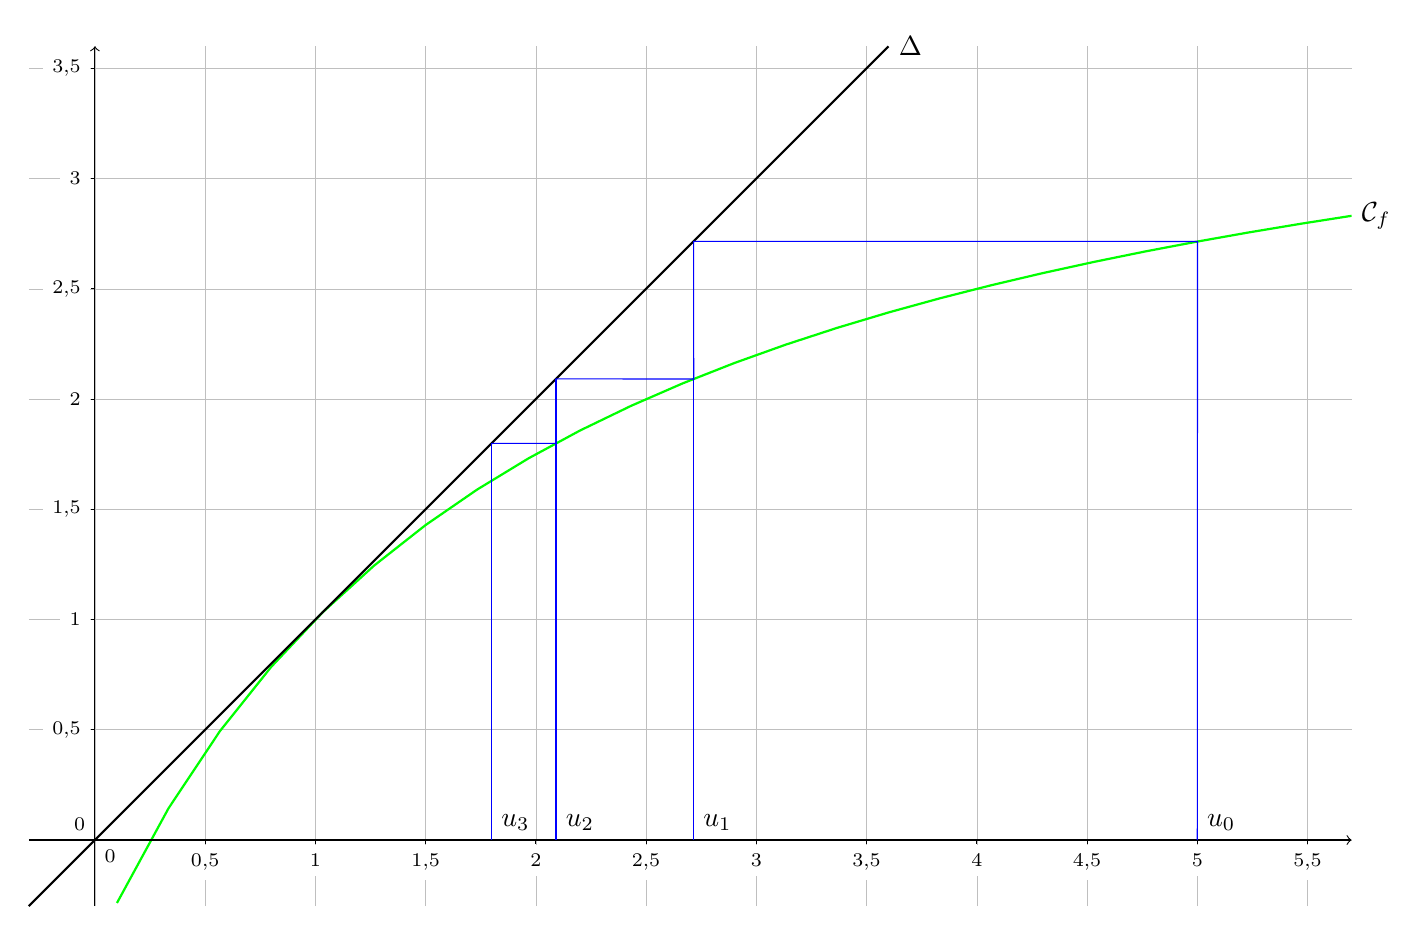
\begin{tikzpicture}[scale=2.8]
  \draw[very thin, lightgray] (-0.3,-0.3) grid [step=0.5] (5.7,3.6) ;
  \draw[thick,green,name path=f] plot [domain=0.1:5.7]
  (\x,{(4*\x-1)/(\x+2)}) node [right,black] { $\mathcal{C}_f$
  } ;
  \draw[thick,name path= D] plot [domain=-0.3:3.6] (\x,\x)
  node[right] { $\Delta$ } ;
  \draw[->] (-0.3,0) -- (5.7,0) ; \draw [->] (0,-0.3) -- (0,3.6) ;
  \foreach \x in {0.5,1,...,5.5} {
    \draw (\x,0) -- (\x,-0.02) node [below,fill=white] {
    \scriptsize \np{\x} } ;
  }
  \foreach \y in {0.5,1,...,3.5} {
    \draw (0,\y) -- (-0.02,\y) node [left,fill=white] {
    \scriptsize \np{\y} } ;
  }
  \draw (0,0) node[below right] { \scriptsize 0} ;
  \draw (0,0) node[above left] { \scriptsize 0} ;

  % construction réponse
  \newdimen\posy
  \newdimen\posx
  \path [name path = u0] (5,0) -- (5,3) ;
  \path [name intersections = {of = f and u0 }] ;
  \coordinate (A) at (intersection-1) ;
  \pgfextracty{\posy}{\pgfpointanchor{A}{center}}
  \path [name path=fu0] (A) -- (0,\posy) ;
  \path [name intersections = {of = fu0 and D}] ;
  \coordinate (B) at (intersection-1) ;
  \pgfextractx{\posx}{\pgfpointanchor{B}{center}}
  \draw[blue,name path=u1] (B) -- (\posx,0) node [above right,
   black] {$u_1$};
  \path [name intersections = {of = u1 and f}] ;
  \coordinate (C) at (intersection-1) ;
  \pgfextracty{\posy}{\pgfpointanchor{C}{center}}
  \path [name path = fu1] (C) -- (0,\posy) ;
  \path [name intersections = {of = fu1 and D}] ;
  \coordinate (D) at (intersection-1) ;
  \pgfextractx{\posx}{\pgfpointanchor{D}{center}}
  \draw[blue,name path=u2] (D) -- (\posx,0) node [above right,
   black] {$u_2$};
  \path [name intersections = {of = u2 and f}] ;
  \coordinate (E) at (intersection-1) ;
  \pgfextracty{\posy}{\pgfpointanchor{E}{center}}
  \path [name path=fu2 ] (E) -- (0,\posy) ;
  \path [name intersections = {of = fu2 and D}] ;
  \coordinate (F) at (intersection-1) ;
  \pgfextractx{\posx}{\pgfpointanchor{F}{center}}
  \draw[blue,name path=u3] (F) -- (\posx,0) node [above right,
   black] {$u_3$} ;


  \draw[blue] (5,0) node [above right,  black] {$u_0$} -- (A)
  -- (B) -- (C) -- (D) -- (E) -- (F) ;
\end{tikzpicture}
\hfill~
\end{Answer}

\pagebreak

\begin{Answer}[number=2]
  \begin{enumerate}
    \item ~\\
      \begin{center}
        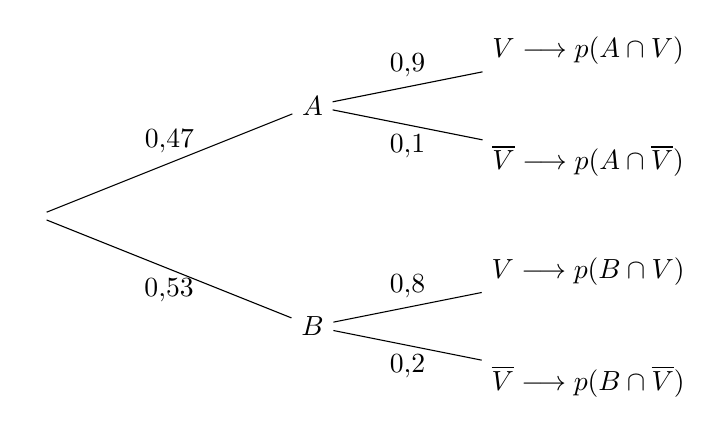
\begin{tikzpicture}[scale=1.4,level distance=25mm,sibling distance=10mm]
          \node {} [grow=right]
          child[sibling distance=20mm] {
            node {$B$}
            child[sibling distance=10mm] {
              node {$\overline{V} \longrightarrow p(B\cap\overline{V})$}
              edge from parent node[below] {$\np{0.2}$}
            }
            child[sibling distance=10mm] {
              node {$V \longrightarrow p(B \cap V)$}
              edge from parent node[above] {$\np{0.8}$}
            }
            edge from parent node[below] { $\np{0.53}$ }
          }
          child[sibling distance=20mm] { node {$A$}
            child[sibling distance=10mm] {
              node {$\overline{V} \longrightarrow p(A\cap\overline{V})$}
              edge from parent node[below] { $\np{0.1}$ }
            }
            child[sibling distance=10mm] {
              node {$V \longrightarrow p(A\cap V)$}
              edge from parent node[above] { $\np{0.9}$ }
            }
            edge from parent node[above] { $\np{0.47}$ }
          } ;
        \end{tikzpicture}
      \end{center}
    \item \begin{enumerate}
        \item \np{0.847}
        \item \np{0.4994}
      \end{enumerate}
    \item $p(A\cap V) + p(B\cap \overline{V})$
  \end{enumerate}
\end{Answer}

\begin{Answer}[number=3]
  \begin{enumerate}
    \item \begin{enumerate}
        \item \begin{itemize}
            \item $u_1 = \frac25 +3 = \frac{17}5 \geqslant
              \frac{15}4\times \np{0.5} = \frac{15}{8}$ ($u_1 \geqslant
              3$ et $\frac{15}8 \leqslant 2$)
            \item $u_n \geqslant \frac{15}4 \times \np{0.5}^n \implies
              \frac15 u_n \geqslant \frac34 \times \np{0.5}^n \implies
              u_{n+1} \geqslant \frac34 \times \np{0.5}^n + 3 \times
              \np{0.5}^n = \frac{15}4 \times \np{0.5}^n \geqslant
              \frac{15}4 \times \np{0.5}^{n+1}$
          \end{itemize}
        \item $u_{n+1} - u_n = \frac{-4}5u_n + 3 \times \np{0.5}^n
          \geqslant \frac{-4}5\times \frac{15}4 \times \np{0.5}^n + 3
          \times \np{0.5}^n = 0$
        \item $u_n$ décroissante minorée, donc convergente.
      \end{enumerate}
    \item \begin{enumerate}
        \item $v_n = u_n - 10\times \np{0.5}^n \implies v_0 = -8$.

          $v_n+1 = u_{n+1} - 10 \times \np{0.5}^{n+1} = \frac15 u_n + 3
          \times \np{0.5}^n - 5 \times \np{0.5}^n = \frac15 u_n -2
          \times \np{0.5}^n = \frac15 v_n$

        \item $v_n = -8\left(\frac15\right)^n$

          $u_n = v_n + 10\times \np{0.5}^n = -8\left(\frac15\right)^n
          +10\times \np{0.5}^n$

        \item $\lim_{n\to+\infty} u_n = 0$
      \end{enumerate}
  \end{enumerate}
\end{Answer}

\end{document}
